% Options for packages loaded elsewhere
\PassOptionsToPackage{unicode}{hyperref}
\PassOptionsToPackage{hyphens}{url}
\PassOptionsToPackage{dvipsnames,svgnames,x11names}{xcolor}
%
\documentclass[
  letterpaper,
  DIV=11,
  numbers=noendperiod]{scrartcl}

\usepackage{amsmath,amssymb}
\usepackage{iftex}
\ifPDFTeX
  \usepackage[T1]{fontenc}
  \usepackage[utf8]{inputenc}
  \usepackage{textcomp} % provide euro and other symbols
\else % if luatex or xetex
  \usepackage{unicode-math}
  \defaultfontfeatures{Scale=MatchLowercase}
  \defaultfontfeatures[\rmfamily]{Ligatures=TeX,Scale=1}
\fi
\usepackage{lmodern}
\ifPDFTeX\else  
    % xetex/luatex font selection
\fi
% Use upquote if available, for straight quotes in verbatim environments
\IfFileExists{upquote.sty}{\usepackage{upquote}}{}
\IfFileExists{microtype.sty}{% use microtype if available
  \usepackage[]{microtype}
  \UseMicrotypeSet[protrusion]{basicmath} % disable protrusion for tt fonts
}{}
\makeatletter
\@ifundefined{KOMAClassName}{% if non-KOMA class
  \IfFileExists{parskip.sty}{%
    \usepackage{parskip}
  }{% else
    \setlength{\parindent}{0pt}
    \setlength{\parskip}{6pt plus 2pt minus 1pt}}
}{% if KOMA class
  \KOMAoptions{parskip=half}}
\makeatother
\usepackage{xcolor}
\setlength{\emergencystretch}{3em} % prevent overfull lines
\setcounter{secnumdepth}{-\maxdimen} % remove section numbering
% Make \paragraph and \subparagraph free-standing
\ifx\paragraph\undefined\else
  \let\oldparagraph\paragraph
  \renewcommand{\paragraph}[1]{\oldparagraph{#1}\mbox{}}
\fi
\ifx\subparagraph\undefined\else
  \let\oldsubparagraph\subparagraph
  \renewcommand{\subparagraph}[1]{\oldsubparagraph{#1}\mbox{}}
\fi


\providecommand{\tightlist}{%
  \setlength{\itemsep}{0pt}\setlength{\parskip}{0pt}}\usepackage{longtable,booktabs,array}
\usepackage{calc} % for calculating minipage widths
% Correct order of tables after \paragraph or \subparagraph
\usepackage{etoolbox}
\makeatletter
\patchcmd\longtable{\par}{\if@noskipsec\mbox{}\fi\par}{}{}
\makeatother
% Allow footnotes in longtable head/foot
\IfFileExists{footnotehyper.sty}{\usepackage{footnotehyper}}{\usepackage{footnote}}
\makesavenoteenv{longtable}
\usepackage{graphicx}
\makeatletter
\def\maxwidth{\ifdim\Gin@nat@width>\linewidth\linewidth\else\Gin@nat@width\fi}
\def\maxheight{\ifdim\Gin@nat@height>\textheight\textheight\else\Gin@nat@height\fi}
\makeatother
% Scale images if necessary, so that they will not overflow the page
% margins by default, and it is still possible to overwrite the defaults
% using explicit options in \includegraphics[width, height, ...]{}
\setkeys{Gin}{width=\maxwidth,height=\maxheight,keepaspectratio}
% Set default figure placement to htbp
\makeatletter
\def\fps@figure{htbp}
\makeatother
\newlength{\cslhangindent}
\setlength{\cslhangindent}{1.5em}
\newlength{\csllabelwidth}
\setlength{\csllabelwidth}{3em}
\newlength{\cslentryspacingunit} % times entry-spacing
\setlength{\cslentryspacingunit}{\parskip}
\newenvironment{CSLReferences}[2] % #1 hanging-ident, #2 entry spacing
 {% don't indent paragraphs
  \setlength{\parindent}{0pt}
  % turn on hanging indent if param 1 is 1
  \ifodd #1
  \let\oldpar\par
  \def\par{\hangindent=\cslhangindent\oldpar}
  \fi
  % set entry spacing
  \setlength{\parskip}{#2\cslentryspacingunit}
 }%
 {}
\usepackage{calc}
\newcommand{\CSLBlock}[1]{#1\hfill\break}
\newcommand{\CSLLeftMargin}[1]{\parbox[t]{\csllabelwidth}{#1}}
\newcommand{\CSLRightInline}[1]{\parbox[t]{\linewidth - \csllabelwidth}{#1}\break}
\newcommand{\CSLIndent}[1]{\hspace{\cslhangindent}#1}

\usepackage{booktabs}
\usepackage{longtable}
\usepackage{array}
\usepackage{multirow}
\usepackage{wrapfig}
\usepackage{float}
\usepackage{colortbl}
\usepackage{pdflscape}
\usepackage{tabu}
\usepackage{threeparttable}
\usepackage{threeparttablex}
\usepackage[normalem]{ulem}
\usepackage{makecell}
\usepackage{xcolor}
\KOMAoption{captions}{tableheading}
\makeatletter
\makeatother
\makeatletter
\makeatother
\makeatletter
\@ifpackageloaded{caption}{}{\usepackage{caption}}
\AtBeginDocument{%
\ifdefined\contentsname
  \renewcommand*\contentsname{Table of contents}
\else
  \newcommand\contentsname{Table of contents}
\fi
\ifdefined\listfigurename
  \renewcommand*\listfigurename{List of Figures}
\else
  \newcommand\listfigurename{List of Figures}
\fi
\ifdefined\listtablename
  \renewcommand*\listtablename{List of Tables}
\else
  \newcommand\listtablename{List of Tables}
\fi
\ifdefined\figurename
  \renewcommand*\figurename{Figure}
\else
  \newcommand\figurename{Figure}
\fi
\ifdefined\tablename
  \renewcommand*\tablename{Table}
\else
  \newcommand\tablename{Table}
\fi
}
\@ifpackageloaded{float}{}{\usepackage{float}}
\floatstyle{ruled}
\@ifundefined{c@chapter}{\newfloat{codelisting}{h}{lop}}{\newfloat{codelisting}{h}{lop}[chapter]}
\floatname{codelisting}{Listing}
\newcommand*\listoflistings{\listof{codelisting}{List of Listings}}
\makeatother
\makeatletter
\@ifpackageloaded{caption}{}{\usepackage{caption}}
\@ifpackageloaded{subcaption}{}{\usepackage{subcaption}}
\makeatother
\makeatletter
\@ifpackageloaded{tcolorbox}{}{\usepackage[skins,breakable]{tcolorbox}}
\makeatother
\makeatletter
\@ifundefined{shadecolor}{\definecolor{shadecolor}{rgb}{.97, .97, .97}}
\makeatother
\makeatletter
\makeatother
\makeatletter
\makeatother
\ifLuaTeX
  \usepackage{selnolig}  % disable illegal ligatures
\fi
\IfFileExists{bookmark.sty}{\usepackage{bookmark}}{\usepackage{hyperref}}
\IfFileExists{xurl.sty}{\usepackage{xurl}}{} % add URL line breaks if available
\urlstyle{same} % disable monospaced font for URLs
\hypersetup{
  pdftitle={Spread Paper Revisions},
  pdfauthor={JMG},
  colorlinks=true,
  linkcolor={blue},
  filecolor={Maroon},
  citecolor={Blue},
  urlcolor={Blue},
  pdfcreator={LaTeX via pandoc}}

\title{Spread Paper Revisions}
\usepackage{etoolbox}
\makeatletter
\providecommand{\subtitle}[1]{% add subtitle to \maketitle
  \apptocmd{\@title}{\par {\large #1 \par}}{}{}
}
\makeatother
\subtitle{Statistical Analysis}
\author{JMG}
\date{}

\begin{document}
\maketitle
\ifdefined\Shaded\renewenvironment{Shaded}{\begin{tcolorbox}[frame hidden, interior hidden, breakable, borderline west={3pt}{0pt}{shadecolor}, boxrule=0pt, enhanced, sharp corners]}{\end{tcolorbox}}\fi

\hypertarget{statistical-analysis-to-determine-relevance-of-factors}{%
\subsection{Statistical analysis to determine relevance of
factors}\label{statistical-analysis-to-determine-relevance-of-factors}}

For a statistical test of our hypothesis, we have use R version 4.3.1
and package \texttt{mgcv} version 1.9 to fit a generalized additive
model (\protect\hyperlink{ref-rcore}{R Core Team 2023};
\protect\hyperlink{ref-wood2003}{S. N. Wood 2003};
\protect\hyperlink{ref-wood2017generalized}{Simon N. Wood 2017}).
Specifically, we model the log odds of county infestation in 2021 with
tensor product smoothing for longitude and latitude to control for
spatial autocorrelation and parametric terms for presence/absence of
two-digit interstate highway, number of garden centers, 2019 county
population, and an interaction term for presence/absence of two-digit
interstate highway and number of garden centers. To deal with issues of
convergence and variables of different scale, we log transformed the
population and normalized the number of garden centers. We used the
packages \texttt{DHARMa} version 0.4.6 and \texttt{gratia} gratia
version 0.8.1.34 for diagnostics to assess model assumptions
(\protect\hyperlink{ref-dharma2022}{Hartig 2022} ;
\protect\hyperlink{ref-gratia2023}{Simpson 2023}).

Figure~\ref{fig-estimates} shows the estimates on the odds-ratio scale
for the parametric terms in our generalized additive logistic regression
model while Table~\ref{tbl-mod-summ} displays the values for the same
estimated coefficients on the log-odds scale. The model results indicate
that the data provides evidence for the increase in likelihood of
infestation in a county in 2021 with the presence of interstate highways
and larger populations. Additionally, our statistical analysis also
suggests that the data provides evidence for the increase in likelihood
of infestation in a county in 2021 with an increase in the number of
garden centers only when there is also the presence of a two-digit
interstate highway for that county.

\begin{figure}

{\centering 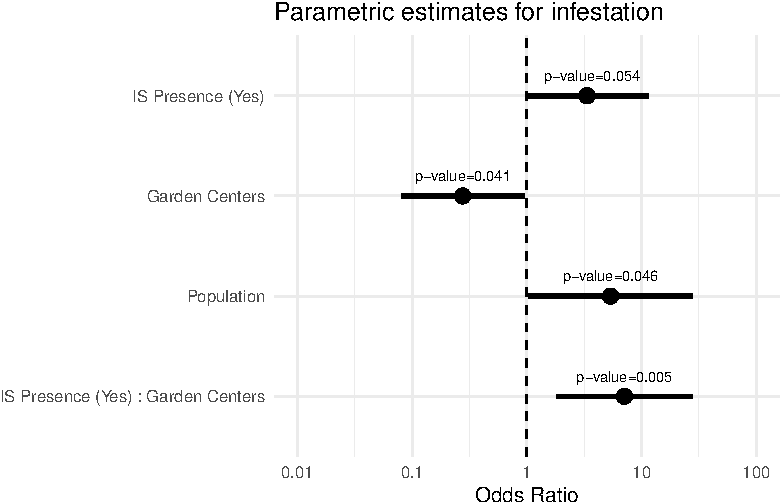
\includegraphics{revisions_statistical_analysis_files/figure-pdf/fig-estimates-1.pdf}

}

\caption{\label{fig-estimates}Estimated coefficients for the linear
predictors in the generalized additive model. Results are on the scale
of odds-ratio. The likelihood of infestation for a county in 2021 is
predicted to increase with the presence of interstate highways and
larger populations. Interestingly, the likelihood of infestation for a
county in 2021 is predicted to increase with an increase in the number
of garden centers only when there is also the presence of a two-digit
interstate highway for that county.}

\end{figure}

\hypertarget{tbl-mod-summ}{}
\begin{table}
\caption{\label{tbl-mod-summ}Summary table for estimates for linear terms in generalized additive
model. Results are on the log-odds scale. }\tabularnewline

\centering
\begin{tabular}{l|r|r|r}
\hline
Coefficient & Estimate & SE & p-value\\
\hline
Intercept & -8.794628 & 4.2781470 & 0.0398105\\
\hline
IS Presence - Yes & 1.207274 & 0.6253652 & 0.0535437\\
\hline
Garden Centers & -1.286439 & 0.6280036 & 0.0405151\\
\hline
Population (log) & 1.679994 & 0.8431980 & 0.0463264\\
\hline
IS Presence - Yes : Garden Centers & 1.959781 & 0.6944467 & 0.0047714\\
\hline
\end{tabular}
\end{table}

\hypertarget{supplementary-analysis}{%
\subsection{Supplementary analysis}\label{supplementary-analysis}}

Figure~\ref{fig-figure-1} displays the 2021 infestation status for the
166 Mid-Atlantic region counties in 2021:

\begin{figure}

{\centering 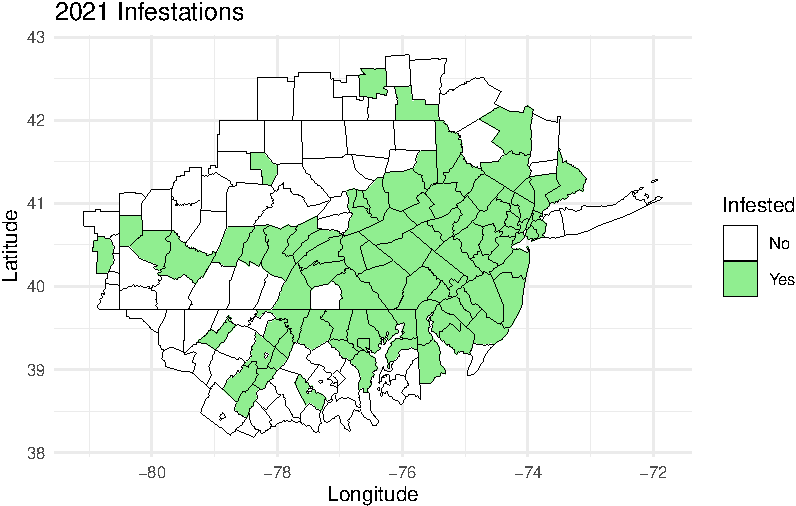
\includegraphics{revisions_statistical_analysis_files/figure-pdf/fig-figure-1-1.pdf}

}

\caption{\label{fig-figure-1}Counties in the defined Mid-Atlantic
regions that were designated as infested by the spotted laternfly in
2021.}

\end{figure}

Table~\ref{tbl-infestations} displays the number of counties per year in
the defined Mid-Atlantic region of 166 that were listed as infected.

\hypertarget{tbl-infestations}{}
\begin{table}
\caption{\label{tbl-infestations}The number of counties per year in the defined Mid-Atlantic region of
166 that were listed as infected. }\tabularnewline

\centering
\begin{tabular}{r|r}
\hline
Year & Number Infested\\
\hline
2014 & 1\\
\hline
2015 & 4\\
\hline
2016 & 6\\
\hline
2017 & 6\\
\hline
2018 & 18\\
\hline
2019 & 26\\
\hline
2020 & 50\\
\hline
2021 & 88\\
\hline
\end{tabular}
\end{table}

Figure~\ref{fig-figure-3} shows the 166 counties in the defined
Mid-Atlantic region together with their 2021 infestation status and the
number of two-digit interstate highways that transect the county.

\begin{figure}

{\centering 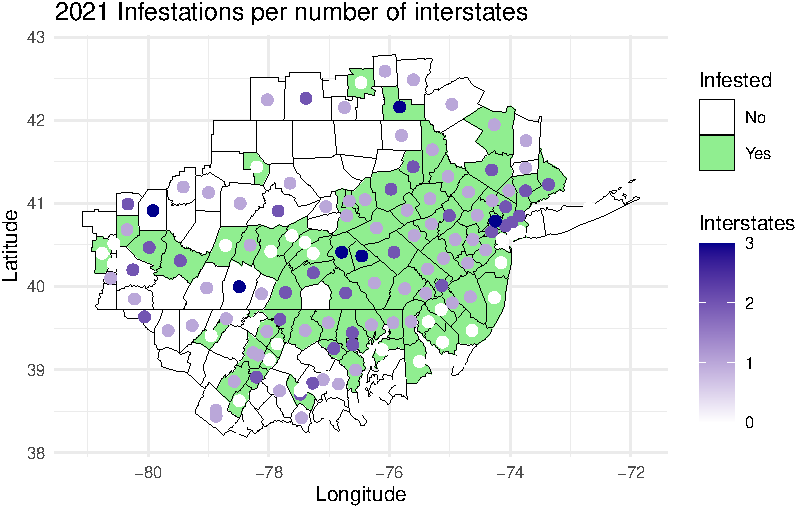
\includegraphics{revisions_statistical_analysis_files/figure-pdf/fig-figure-3-1.pdf}

}

\caption{\label{fig-figure-3}Spotted laternfly infested counties for
2021 together with the number of two-digit interstate highways
transecting the counties.}

\end{figure}

Figure~\ref{fig-figure-4} shows the 166 counties in the defined
Mid-Atlantic region together with their 2021 infestation status and the
number of garden centers in the county.

\begin{figure}

{\centering 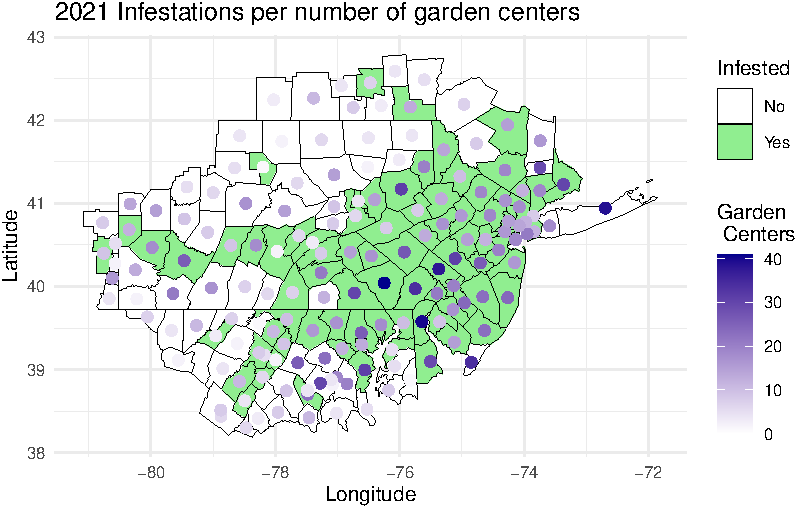
\includegraphics{revisions_statistical_analysis_files/figure-pdf/fig-figure-4-1.pdf}

}

\caption{\label{fig-figure-4}Spotted laternfly infested counties for
2021 together with the number of garden centers in the counties.}

\end{figure}

Figure~\ref{fig-figure-5} shows the 166 counties in the defined
Mid-Atlantic region together with their 2021 infestation status and the
county population on the log scale as estimated in 2019.

\begin{figure}

{\centering 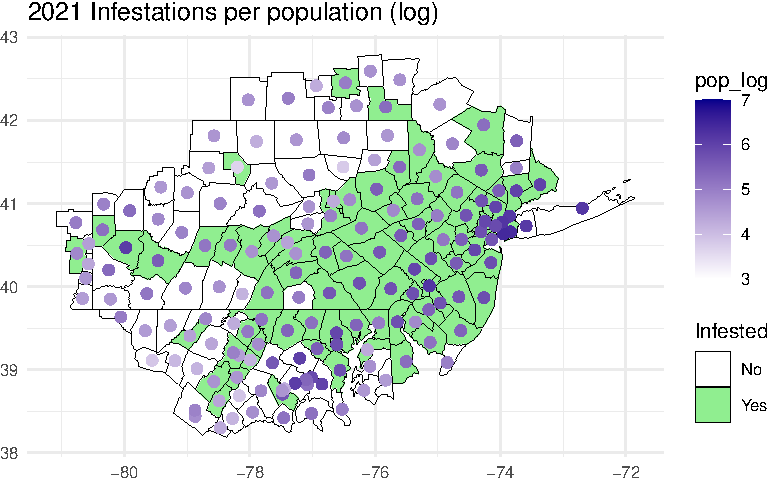
\includegraphics{revisions_statistical_analysis_files/figure-pdf/fig-figure-5-1.pdf}

}

\caption{\label{fig-figure-5}Spotted laternfly infested counties for
2021 together with the 2019 estimated population (log scale) for the
counties.}

\end{figure}

Figure~\ref{fig-figure-6} shows the 166 counties in the defined
Mid-Atlantic region together with the presence/absence of two-digit
interstate highways and the number of garden center per county.

\begin{figure}

{\centering 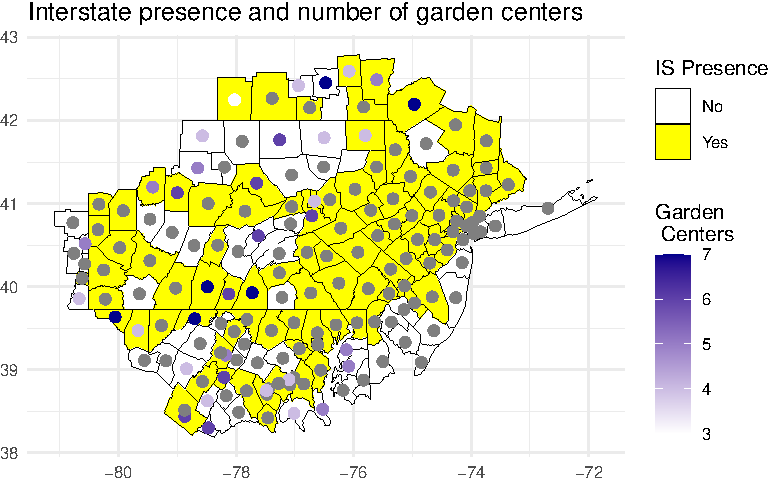
\includegraphics{revisions_statistical_analysis_files/figure-pdf/fig-figure-6-1.pdf}

}

\caption{\label{fig-figure-6}Spotted laternfly infested counties for
2021 together with the presence/absence of two-digit interstate highways
and the number of garden center per county.}

\end{figure}

\hypertarget{infestation-trend-over-time}{%
\subsubsection{Infestation Trend Over
Time}\label{infestation-trend-over-time}}

(\protect\hyperlink{ref-gratia2023}{Simpson 2023})

\begin{figure}

{\centering 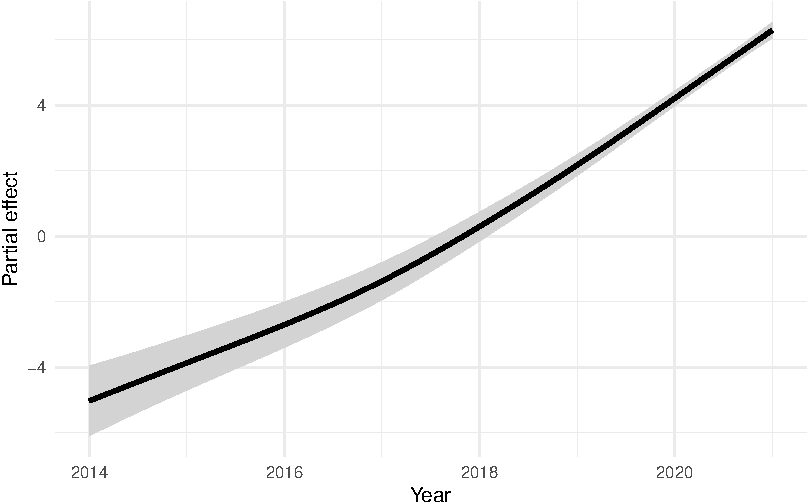
\includegraphics{revisions_statistical_analysis_files/figure-pdf/fig-time-1.pdf}

}

\caption{\label{fig-time}Partial effect plot for the log odds of
infestation over time from 2014 - 2021.}

\end{figure}

\begin{figure}

{\centering 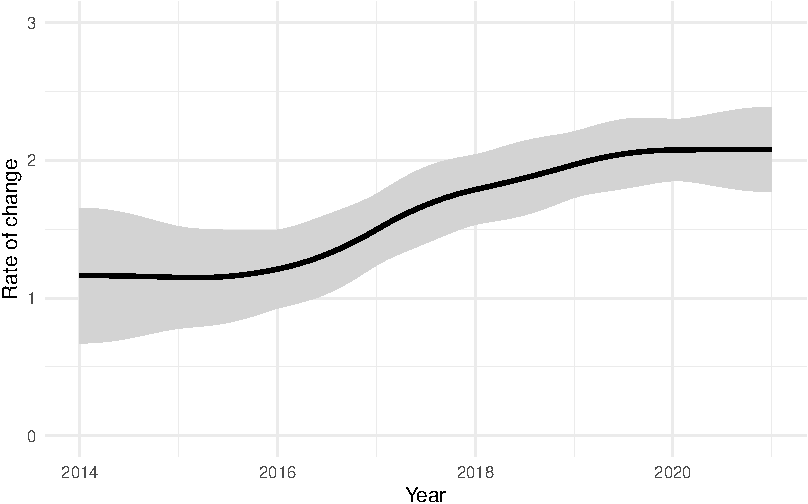
\includegraphics{revisions_statistical_analysis_files/figure-pdf/fig-time-deriv-1.pdf}

}

\caption{\label{fig-time-deriv}Time rate of change (i.e., first
derivative) of partial effect of the log odds of infestation over time
from 2014 - 2021.}

\end{figure}

\hypertarget{references}{%
\subsection{References}\label{references}}

\hypertarget{refs}{}
\begin{CSLReferences}{1}{0}
\leavevmode\vadjust pre{\hypertarget{ref-dharma2022}{}}%
Hartig, Florian. 2022. \emph{DHARMa: Residual Diagnostics for
Hierarchical (Multi-Level / Mixed) Regression Models}.
\url{https://CRAN.R-project.org/package=DHARMa}.

\leavevmode\vadjust pre{\hypertarget{ref-rcore}{}}%
R Core Team. 2023. \emph{R: A Language and Environment for Statistical
Computing}. Vienna, Austria: R Foundation for Statistical Computing.
\url{https://www.R-project.org/}.

\leavevmode\vadjust pre{\hypertarget{ref-gratia2023}{}}%
Simpson, Gavin L. 2023. \emph{{gratia}: Graceful {ggplot}-Based Graphics
and Other Functions for {GAM}s Fitted Using {mgcv}}.
\url{https://gavinsimpson.github.io/gratia/}.

\leavevmode\vadjust pre{\hypertarget{ref-wood2003}{}}%
Wood, S. N. 2003. {``Thin-Plate Regression Splines.''} \emph{Journal of
the Royal Statistical Society (B)} 65 (1): 95--114.

\leavevmode\vadjust pre{\hypertarget{ref-wood2017generalized}{}}%
Wood, Simon N. 2017. \emph{Generalized Additive Models: An Introduction
with r}. CRC press.

\end{CSLReferences}



\end{document}
